\documentclass[12pt,titlepage]{article}
\usepackage[margin=1.25in]{geometry}
\usepackage{graphicx,amsmath,blindtext,minted}

%% Variables definition
\newcommand{\vSubject}{Mathematics 3}
\newcommand{\vSubtitle}{Distance Measures for Machine Learning}
\newcommand{\vName}{Muhammad Baihaqi Aulia Asy'ari}
\newcommand{\vNIM}{2241720145}
\newcommand{\vClass}{2I}
\newcommand{\vDepartment}{Information Technology}
\newcommand{\vStudyProgram}{D4 Informatics Engineering}

%% [START] Tikz related stuff
\usepackage{tikz}
\usetikzlibrary{svg.path,calc,shapes.geometric,shapes.misc}
\tikzstyle{terminator} = [rectangle, draw, text centered, rounded corners = 1em, minimum height=2em]
\tikzstyle{preparation} = [chamfered rectangle, chamfered rectangle sep=0.75em, draw, text centered, minimum height = 2em]
\tikzstyle{process} = [rectangle, draw, text centered, minimum height=2em]
\tikzstyle{decision} = [diamond, aspect=2, draw, text centered, minimum height=2em]
\tikzstyle{data}=[trapezium, draw, text centered, trapezium left angle=60, trapezium right angle=120, minimum height=2em]
\tikzstyle{connector} = [line width=0.25mm,->]
%% [END] Tikz related stuff

%% [START] Fancy header related stuff
\usepackage{fancyhdr}
\pagestyle{fancy}
\setlength{\headheight}{15pt} % compensate fancyhdr style
\fancyhead{}
\fancyfoot{}
\fancyfoot[L]{\thepage}
\fancyfoot[R]{\textit{\vSubject - \vSubtitle}}
\renewcommand{\footrulewidth}{0.4pt}% default is 0pt, overline for footer
%% [END] Fancy header related stuff

%% [START] Custom tabular command related stuff
\usepackage{tabularx}
\newcommand{\details}[2]{
    #1 & #2  \\
}
%% [END] Custom tabular command related stuff

%% [START] Figure related stuff
\newcommand{\image}[3][1]{
    \begin{figure}[h]
        \centering
        \includegraphics[#1]{#2}
        \caption{#3}
        \label{#3}
    \end{figure}
}
%% [END] Figure related stuff

%%
\usepackage{pgf-umlcd}

\renewcommand{\umldrawcolor}{black}
\renewcommand{\umlfillcolor}{white}
%%

%% [BEGIN] Custom enumerator
\usepackage{enumitem}
%% [END] Custom enumerator

%% [BEGIN] Paragraph indent
\usepackage{indentfirst}
%% [END] Paragraph indent

\begin{document}
\begin{titlepage}
    \centering
    \vfill
    {\bfseries\LARGE
        \vSubject\\
        \vskip0.25cm
        \vSubtitle
    }
    \vfill
    
\includegraphics[width=6cm]{images/polinema-logo.png}
    \vfill
    {
        \textbf{Name}\\
        \vName\\
        \vskip0.5cm
        \textbf{NIM}\\
        \vNIM\\
        \vskip0.5cm
        \textbf{Class}\\
        \vClass\\
        \vskip0.5cm
        \textbf{Department}\\
        \vDepartment\\
        \vskip0.5cm
        \textbf{Study Program}\\
        \vStudyProgram
    }
\end{titlepage}

\newpage

\section*{Task 1}

\includegraphics[width=\textwidth]{images/figures/fig2.png}

\begin{align*}
    9 &= 1001 \\
    14 &= 1110 \\
    &= 0111 \\
    &= 3
\end{align*}

\section*{Task 2}

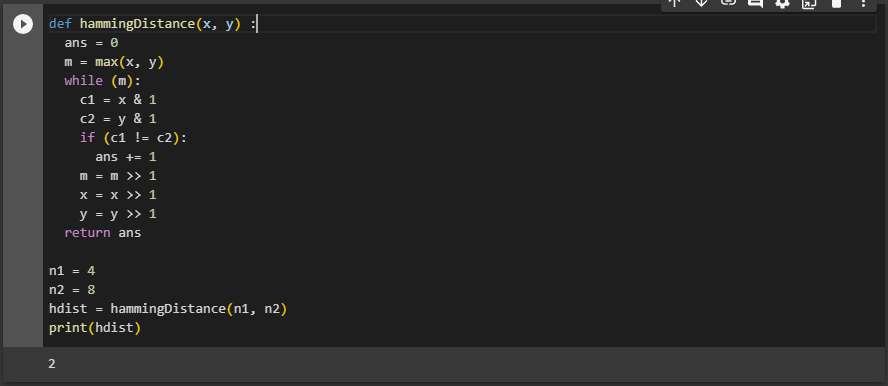
\includegraphics[width=\textwidth]{images/figures/fig3.png}

\newpage

\section*{Additional Task}

\begin{enumerate}
    \item count the hamming distance of these
    \begin{center}
        BEEN\\
        BEAN\\
        0010
    \end{center}
    \begin{center}
        CEREAL\\
        SERIAL\\
        100100
    \end{center}
    hamming distance of BEEN and BEAN is 1\\
    hamming distance of CEREAL and SERIAL is 2
    \item hamming distance from 10 and 15 (binary)
    \begin{align*}
        10 &= 1010\\
        15 &= 1111\\
        &= 0101\\
        &= 2
    \end{align*}
    \item hamming distance from 6 and 11 (binary)
    \begin{align*}
        6 &= 0110\\
        11 &= 1011\\
        &= 1101\\
        &= 3
    \end{align*}
\end{enumerate}

\newpage

\section*{Task 3}

\begin{minted}[autogobble,breaklines,linenos]{python3}
    from math import sqrt

    def minkowski_distance(a, b, p):
    return sum(abs(e1-e2)**p for e1, e2 in zip(a,b))**(1/p)

    row1 = [10, 20, 15, 10, 5]
    row2 = [12, 24, 18, 8, 7]

    dist = minkowski_distance(row1, row2, 1)
    print(dist)

    dist = minkowski_distance(row1, row2, 2)
    print(dist)
\end{minted}

\includegraphics[width=\textwidth]{images/figures/fig1.png}

p = 1
\begin{align*}
    d(x,y) &= (|10-12|^1+|20-24|^1+|15-18|^1+|10-8|^1+|5-7|^1)^{(1/1)} \\
    &= (|2|^1+|4|^1+|3|^1+|2|^1+|2|^1)^{1} \\
    &= (2+4+3+2+2) \\
    &= 13 \\
\end{align*}

p = 2
\begin{align*}
    d(x,y) &= (|10-12|^2+|20-24|^2+|15-18|^2+|10-8|^2+|5-7|^2)^{(1/2)} \\
    &= \sqrt{(|2|^2+|4|^2+|3|^2+|2|^2+|2|^2)} \\
    &= \sqrt{(4+16+9+4+4)} \\
    &= \sqrt{37} = 6.082\\
\end{align*}

\newpage

\section*{Task 4}

\subsection*{A Resume on Minkowski and Chebyshev Distance}
The Minkowski distance is a mathematical tool used to measure how far apart two sets of numbers are from each other. It's like a flexible ruler that can be adjusted based on a special number called "order" or p. This allows us to calculate distances in different ways depending on the situation. So, Minkowski distance is a helpful tool in math and data analysis that lets us customize how we measure distances to fit our needs.

Chebyshev's distance is a metric used to quantify the dissimilarity between two points in a grid or vector space. It measures the maximum absolute difference between corresponding coordinates of these points it provides a straightforward way to gauge the "worst-case scenario" for movement between two points within a multi-dimensional space.

Minkowski's mathematical equation goes as follows
\begin{equation*}
    \sqrt[r]{\sum_{k=1}^{n}|x_k-y_k|^r}
\end{equation*}

Chebyshev's mathematical equation goes as follows
\begin{equation*}
    \lim_{q\rightarrow\infty}\sqrt[r]{\sum_{i=1}^{n}|x_i-y_i|^q}
\end{equation*}

Minkowski distance plays a vital role in portfolio diversification. Minkowski distance helps with this by measuring their similarity. A larger distance indicates that these assets have distinct risk and return characteristics, making them suitable for diversification.

In the world of financial security, Chebyshev distance is a useful tool for making fraud detection better. This metric allows us to pinpoint potential irregularities by measuring the most significant deviation between transaction attributes. When integrated into machine learning models and real-time monitoring systems, it aids in swiftly flagging transactions that fall beyond predefined thresholds.
\end{document}